\section{Charactersitics of \rt{} transit data}
\label{sec:realtime-data}

There are a range of \gls{avl} technologies which allow transit vehicles to report their location in \rt{}. The most common of these is now the \gls{gps}, which provides the longitude and latitude of the vehicle. In the simplest of deployments, each vehicle reports its location to a central server at a fixed time interval. The server then collates the reports from all of the buses in the fleet and makes them available via an \gls{api}.


Another type of \rt{} data available to us is arrival and departure information at bus stops. When a vehicle arrives at or departs from a stop (or thinks it does), it reports to the server which stop it is at, and its time of arrival or departure. The server then computes the delay (the time between actual and scheduled arrival or departure), collates the data from multiple vehicles, and also makes these available through an \gls{api}.


\Rt{} vehicle information can be displayed in one of two ways. \Gls{gps} positions are displayed on a map accessed through a mobile app, allowing commuters to see where their bus was when it last reported its location. For trip updates, the \emph{current delay} is added to the scheduled arrival time and displayed to commuters, usually as a \emph{time until arrival}, in minutes. The \gls{eta} can be displayed either on a mobile app or, more commonly, on a \rt{} arrivals board located at the stop.


What we have just described is in fact the entirety of \gls{rti} in Auckland and some other transit locations around the world. While at first it seems an adequate solution, discussion with just about any regular public transport user will prove otherwise. The reasons for this become obvious with a little scrutiny, which we will now uncover.
(Note to self: most of this was probably described in the Intro).


\subsection{Vehicle positions}
\label{sec:vp_data}

Every measurement of a data point comes with some associated error. In the case of \gls{gps} devices, this error is usually small with precision depending on the quality of the device. However, it is possible for any device to succumb to several factors which can place the bus far from its intended path, the primary reason being buildings or other obstacles resulting in a poor signal. Surprisingly, however, this is not the main issue with vehicle position data.


Object tracking has been well studied, and many algorithms exist for tracking an object through space using \gls{gps} observations. However, these usually take high-frequency observations (seconds or milliseconds) which can generate an almost exact \rt{} estimate of the objects actual location.


Many examples of \rt{} object tracking exist, however the most relatable to most readers will be in their pocket. When getting directions from your phone, the maps application requests the user's phone's location continuously, providing the exact location with a second or less of delay. However, have you ever been driving along, following directions, when you've suddenly missed the turn off? Often, the maps application will show you as \emph{on course} for several seconds until it realises that you well and truly have gone off track and reroutes your route. This is an example of a \rt{} position tracking algorithm that is attempting to follow the device's location whilst simultaneously accounting for inherent noise in the measurements. When the driver first goes off track, the algorithm assumes this is a measurement error, and lets the vehicle continue on course. Eventually the error becomes large and consistent enough that the model stops assuming the driver is following the planned route.


With \rt{} transit data, the frequency of observations is vastly reduced, with observations obtained anywhere from 10~seconds to a minute (or more) between. This makes it very difficult to estimate the vehicle's exact location. It also means that, on recieving a vehicle position that doesn't seem quite right, it can take another 30~seconds before a second observation is obtained to determine if it was the result of a bad measurement or a real event.


Another major complication with the Auckland Transport vehicle data is that vehicles often report their location when arriving at or departing from a bus stop; \emph{however}, instead of reporting their \gls{gps} location as measured from the \gls{gps} device, they report the location of the bus stop itself, which is known exactly. So, what happens when the bus approaches a bus stop at speed, only to come to a halt at an intersection 100~m before hand? The vehicle's \gls{gps} continues predicting the trajectory and places the vehicle at the bus stop before it actually arrives. This triggers a trip update (section~\ref{sec:tu_data}), which itself produces a vehicle position update \emph{exactly at the bus stop}. However, a passenger standing at the stop will see the bus sitting at the lights, while the \rt{} board displays the bus as having arrived. For the passenger waiting at this stop, this is of no concern, as now they can see the bus and have no need for \rt{} data. For the passengers at stops down the line, however, this can have some frustrating implications. This leads into another phenomenon in which the bus may appear to go backwards according to the sequence of \gps{} coordinates, discussed in detail in \cref{sec:data_issues}. The main consequence of this problem is that within the data processing component of our application, we check for vehicle position updates associated with trip updates and remove them (that is, we use the trip update and not the vehicle position).




\subsection{Trip updates}
\label{sec:tu_data}

As elluded to earlier, trip updates are prone to their own form of measurement error. Without human intervention, it is very difficult for the \gls{gps} tracking system on the bus to determine exactly when the bus arrives at or leaves a bus stop. In situations such as that described above, this can mean the arrival time is reported before the bus actually arrives, resulting in a premature arrival time and, more importantly, \emph{a severly reduced delay}.


Traffic lights may hold up a bus for a minute (or more), so the bus may, for argument sake, appear to arrive exactly on time. The result of this is the propogation of the current delay to all future stops, which then display an \gls{eta} that matches the scheduled arrival time. However, two minutes later, after the bus has finally arrived at the stop, dropped off and picked up passengers, it departs, triggering another trip update. The delay, now two minutes, is propogated to upcoming stops. Passengers waiting at these stops see the \gls{eta} jump suddenly by two minutes, as demonstrated in \cref{fig:tu_eta_jump}, leading inevitably to much frustration for passengers.

\begin{knitrout}\small
\definecolor{shadecolor}{rgb}{0.969, 0.969, 0.969}\color{fgcolor}\begin{figure}

{\centering 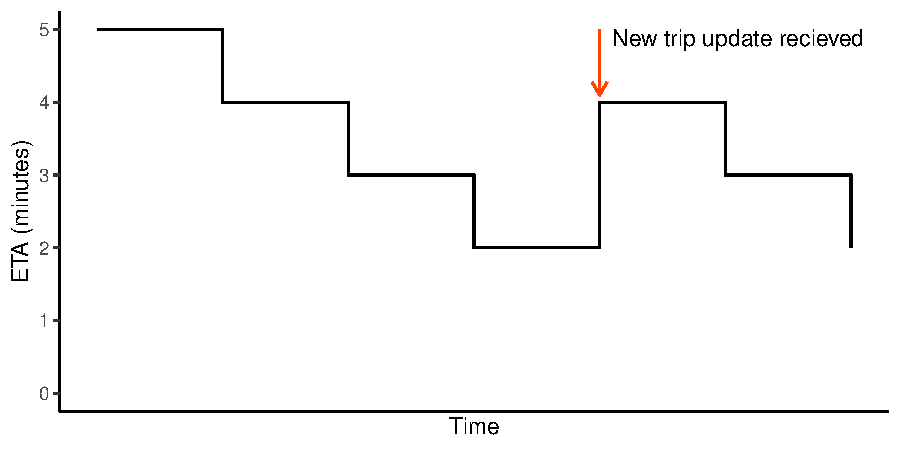
\includegraphics[width=.8\textwidth]{figure/tu_eta_jump-1} 

}

\caption[\glspl{eta}, displayed as integer minutes, decrease over time until new data is recieved, marked by an arrow]{\glspl{eta}, displayed as integer minutes, decrease over time until new data is recieved, marked by an arrow. If the bus has been delayed, the ETA as seen by the passenger may suddenly 'jump'.}\label{fig:tu_eta_jump}
\end{figure}


\end{knitrout}


The reverse can also occur, for example if for some reason the bus reports its arrival or departure late. However, what is more common is that the update is skipped altogether, and so a bus that was 5~minutes behind schedule has made up several minutes and arrives at the bus stop while the \rt{} board still shows it as being 2~minutes away. While this may seem like a good thing---passengers already at the stop have a shorter wait---other passengers making their timely way to the bus may have to sprint the last leg (or miss the bus altogether).


On the data side, the main repercussion of this is that arrival and departure times are very noisy and difficult to trust; however, they provide a lot of information without which it would be almost impossible to infer the trajectory of a bus between stops---which is the primary aim of this part of our work. We discuss this further in \cref{sec:pf-likelihood} when we present the likelihood function.
